\documentclass[a4paper,10pt]{book}
\usepackage[utf8]{inputenc}
\usepackage[spanish]{babel}

\decimalpoint
\usepackage{dcolumn}
\newcolumntype{.}{D{.}{\esperiod}{-1}}
\makeatletter
\addto\shorthandsspanish{\let\esperiod\es@period@code}
\makeatother

\RequirePackage{verbatim}
\usepackage{fancyhdr}
\usepackage{graphicx}
\usepackage{afterpage}
\usepackage{longtable}
\usepackage{hyperref}
\usepackage{url}
\usepackage{colortbl,longtable}
\usepackage[stable]{footmisc}
\usepackage{index}
\usepackage{csquotes}
\usepackage{listings}
\usepackage{xcolor}

\definecolor{codegreen}{rgb}{0,0.6,0}
\definecolor{codegray}{rgb}{0.5,0.5,0.5}
\definecolor{codepurple}{rgb}{0.58,0,0.82}
\definecolor{backcolour}{rgb}{0.95,0.95,0.92}

\lstdefinestyle{mystyle}{
	backgroundcolor=\color{backcolour},   
	commentstyle=\color{codegreen},
	keywordstyle=\color{magenta},
	numberstyle=\tiny\color{codegray},
	stringstyle=\color{codepurple},
	basicstyle=\ttfamily\footnotesize,
	breakatwhitespace=false,         
	breaklines=true,                 
	captionpos=b,                    
	keepspaces=true,                 
	numbers=left,                    
	numbersep=5pt,                  
	showspaces=false,                
	showstringspaces=false,
	showtabs=false,                  
	tabsize=2
}

% \lstset{mystyle}

% Customizar colores de enlaces
\hypersetup{
	colorlinks=true,
	citecolor=blue,
	linkcolor=black,
	filecolor=magenta,
	urlcolor=cyan,
	pdfpagemode=FullScreen
}

% ********************************************************************
% Re-usable information
% ********************************************************************
\newcommand{\myTitle}{Lazarillo - Robot guía: Plataforma robótica de código abierto para uso general.\xspace}
\newcommand{\myDegree}{Máster en Ingeniería Informática\xspace}
\newcommand{\myName}{Adrián Morente Gabaldón\xspace}
\newcommand{\myProf}{Juan José Ramos Muñoz\xspace}
\newcommand{\myFaculty}{Escuela Técnica Superior de Ingenierías Informática y de Telecomunicación\xspace}
\newcommand{\myFacultyShort}{E.T.S. de Ingenierías Informática y de Telecomunicación\xspace}
\newcommand{\myDepartment}{Departamento de ...\xspace}
\newcommand{\myUni}{\protect{Universidad de Granada}\xspace}
\newcommand{\myLocation}{Granada\xspace}
\newcommand{\myTime}{\today\xspace}
\newcommand{\myVersion}{Versión 1.0\xspace}

\hypersetup{
pdfauthor = {\myName (adrian95morente@gmail.com)},
pdftitle = {\myTitle},
pdfsubject = {},
pdfkeywords = {},
pdfcreator = {},
pdfproducer = {pdflatex}
}

%\makeindex
%\usepackage[style=long, cols=2,border=plain,toc=true,number=none]{glossary}
% \makeglossary

% Definición de comandos que me son tiles:
%\renewcommand{\indexname}{Índice alfabético}
%\renewcommand{\glossaryname}{Glosario}

\pagestyle{fancy}
\fancyhf{}
\fancyhead[LO]{\leftmark}
\fancyhead[RE]{\rightmark}
\fancyhead[RO,LE]{\textbf{\thepage}}
\renewcommand{\chaptermark}[1]{\markboth{\textbf{#1}}{}}
\renewcommand{\sectionmark}[1]{\markright{\textbf{\thesection. #1}}}

\setlength{\headheight}{1.5\headheight}

\newcommand{\HRule}{\rule{\linewidth}{0.5mm}}
%Definimos los tipos teorema, ejemplo y definición podremos usar estos tipos
%simplemente poniendo \begin{teorema} \end{teorema} ...
\newtheorem{teorema}{Teorema}[chapter]
\newtheorem{ejemplo}{Ejemplo}[chapter]
\newtheorem{definicion}{Definición}[chapter]

\definecolor{gray97}{gray}{.97}
\definecolor{gray75}{gray}{.75}
\definecolor{gray45}{gray}{.45}
\definecolor{gray30}{gray}{.94}

\lstset{ frame=Ltb,
     framerule=0.5pt,
     aboveskip=0.5cm,
     framextopmargin=3pt,
     framexbottommargin=3pt,
     framexleftmargin=0.1cm,
     framesep=0pt,
     rulesep=.4pt,
     backgroundcolor=\color{gray97},
     rulesepcolor=\color{black},
     %
     stringstyle=\ttfamily,
     showstringspaces = false,
     basicstyle=\scriptsize\ttfamily,
     commentstyle=\color{gray45},
     keywordstyle=\bfseries,
     %
     numbers=left,
     numbersep=6pt,
     numberstyle=\tiny,
     numberfirstline = false,
     breaklines=true,
   }
 
% minimizar fragmentado de listados
\lstnewenvironment{listing}[1][]
   {\lstset{#1}\pagebreak[0]}{\pagebreak[0]}

\lstdefinestyle{CodigoC}
   {
	basicstyle=\scriptsize,
	frame=single,
	language=C,
	numbers=left
   }
\lstdefinestyle{CodigoC++}
   {
	basicstyle=\small,
	frame=single,
	backgroundcolor=\color{gray30},
	language=C++,
	numbers=left
   }
\lstdefinestyle{Consola}
   {basicstyle=\scriptsize\bf\ttfamily,
    backgroundcolor=\color{gray30},
    frame=single,
    numbers=none
   }
\newcommand{\bigrule}{\titlerule[0.5mm]}

%Para conseguir que en las páginas en blanco no ponga cabeceras
\makeatletter
\def\clearpage{%
  \ifvmode
    \ifnum \@dbltopnum =\m@ne
      \ifdim \pagetotal <\topskip
        \hbox{}
      \fi
    \fi
  \fi
  \newpage
  \thispagestyle{empty}
  \write\m@ne{}
  \vbox{}
  \penalty -\@Mi
}
\makeatother

\usepackage{pdfpages}
\begin{document}
\begin{titlepage}

\newlength{\centeroffset}
\setlength{\centeroffset}{-0.5\oddsidemargin}
\addtolength{\centeroffset}{0.5\evensidemargin}
\thispagestyle{empty}

\noindent\hspace*{\centeroffset}\begin{minipage}{\textwidth}

\centering

\includegraphics[width=0.9\textwidth]{imagenes/ugr.png}\\[1.4cm]

\textsc{\Large TRABAJO FIN DE MÁSTER\\[0.2cm]}
\textsc{MÁSTER EN INGENIERÍA INFORMÁTICA}\\[1cm]
% Upper part of the page
% 
% Title
{\Huge\bfseries Lazarillo - Robot guía\\
}
\noindent\rule[-1ex]{\textwidth}{3pt}\\[3.5ex]
{\large\bfseries Plataforma robótica de código abierto para uso general}
\end{minipage}

\vspace{2.5cm}
\noindent\hspace*{\centeroffset}\begin{minipage}{\textwidth}
\centering

\textbf{Autor}\\ {Adrián Morente Gabaldón}\\[2.5ex]
\textbf{Director}\\
{Juan José Ramos Muñoz}\\[2cm]

\includegraphics[width=0.3\textwidth]{imagenes/etsiit_logo.png}\\[0.1cm]
\textsc{Escuela Técnica Superior de Ingenierías Informática y de Telecomunicación}\\
\textsc{---}\\
Granada, septiembre de 2022
\end{minipage}
%\addtolength{\textwidth}{\centeroffset}
%\vspace{\stretch{2}}
\end{titlepage}

\chapter*{}

%\cleardoublepage
\thispagestyle{empty}

\begin{center}
{\large\bfseries Lazarillo - Robot guía: Plataforma robótica de código abierto para uso general}\\
\end{center}
\begin{center}
Adrián Morente Gabaldón\\
\end{center}

%\vspace{0.7cm}
\noindent{\textbf{Palabras clave}: robot, embebido, \textit{IoT}, \textit{Linux}, \textit{Yocto}, web, \textit{C++}, \textit{PubSub}, \textit{React}, \textit{Docker}, \textit{Python}, \textit{Redis}}\\

\vspace{0.7cm}
\noindent{\textbf{Resumen}}\\

Lazarillo se trata de una plataforma libre de código abierto pensada para provisionar un robot que actúa como guía de caminos para los visitantes que acuden a la ETSIIT.\\

Este dispositivo embebido consta de un sistema operativo hecho a medida además de diversas aplicaciones para su uso, e internamente una arquitectura software que permite extender sus funcionalidades a todos los desarrolladores interesados.\\

En cuanto a \textit{IoT}, la plataforma consta de métodos de conectividad que permiten al dispositivo ser administrado por un técnico desde un portal web, pudiendo así realizar actualizaciones o gestiones varias.
\cleardoublepage


\thispagestyle{empty}


\begin{center}
{\large\bfseries Lazarillo - Robot guide: Open-source multipurpose robotic platform}\\
\end{center}
\begin{center}
Adrián Morente Gabaldón\\
\end{center}

%\vspace{0.7cm}
\noindent{\textbf{Keywords}: robot, embedded, \textit{IoT}, \textit{Linux}, \textit{Yocto}, web, \textit{C++}, \textit{PubSub}, \textit{React}, \textit{Docker}, \textit{Python}, \textit{Redis}}\\

\vspace{0.7cm}
\noindent{\textbf{Abstract}}\\

Lazarillo is a free \& open-source platform for provisioning a robot that shall behave as a path guide for the ETSIIT's visitors.\\

This embedded device contains a custom-made operating system in addition to some assorted applications. Internally, it contains a software architecture that allows any interested developers to extend its functionalities.\\

Regarding \textit{IoT}, the platform includes connectivity methods that make a technician able to manage or upgrade the device through a web portal.

\chapter*{}
\thispagestyle{empty}

\noindent\rule[-1ex]{\textwidth}{2pt}\\[4.5ex]

Yo, \textbf{Adrián Morente Gabaldón}, alumno de la titulación Máster en Ingeniería Informática de la \textbf{Escuela Técnica Superior de Ingenierías Informática y de Telecomunicación de la Universidad de Granada}, con DNI 77139229N, autorizo la ubicación de la siguiente copia de mi Trabajo Fin de Grado en la biblioteca del centro para que pueda ser consultada por las personas que lo deseen.

\vspace{6cm}

\noindent Fdo: Adrián Morente Gabaldón

\vspace{2cm}

\begin{flushright}
Granada a 9 de septiembre de 2022.
\end{flushright}

\chapter*{Agradecimientos}
\thispagestyle{empty}

       \vspace{1cm}


Poner aquí agradecimientos...


% \frontmatter
\tableofcontents
%\listoffigures
%\listoftables
% \mainmatter
%\setlength{\parskip}{5pt}

\chapter{Introducción}

\textbf{Lazarillo} se trata de una plataforma robótica abierta cuyo propósito es proporcionar una arquitectura solvente y extensible que permita añadir nuevas características y utilidades, además de facilitar el acceso a su gestión y mantenimiento.\\

Contiene un sistema operativo abierto basado en GNU/Linux y \textit{The Yocto Project}, además de distintos servicios implementados con lenguajes de programación diferentes, mostrando así la interoperabilidad del software. Goza de conectividad inalámbrica, la cual facilita la conexión con herramientas externas para su gestión. Asímismo, el proyecto también consta de un panel web de administración desde el cual se pueden enviar acciones remotas al robot.\\

Aunque se trata de una plataforma extensible y de propósito múltiple, el uso inicial para el que fue ideado es el de actuar como \textbf{asistente} y \textbf{guía} dentro de un espacio cerrado (ya podemos ver que el título asignado al proyecto es un pequeño guiño a la literatura española). Sin embargo, el \textit{stack} de herramientas y arquitectura que se han ido confeccionando durante su desarrollo, se podrían utilizar fácilmente para cualquier proyecto de propósito general que aúne dispositivos embebidos con \textit{IoT} y administración remota de éstos.
\chapter{Estado del arte}

TODO: listar robots existentes, describiendo el grado de extensibilidad de cada uno de ellos

TODO: listar plataformas móviles como la de una Roomba, diciendo por qué no podemos usarla (código cerrado)

TODO: describir sucíntamente ROS y por qué no es necesario usarlo existiendo Redis

TODO: listar placas como RPI

TODO: listar sistemas operativos para RPI como Raspbian

TODO: describir uso de yocto en lugar de Buildroot y otras alternativas
\chapter{Especificación y requisitos}

Pasemos ahora a describir de la forma más detallada posible cada uno de los requerimientos que conforman la idea del proyecto, planteando del mismo modo alternativas o aspectos que sería de agrado incluir, si bien no forman parte de la especificación inicialmente. Las decisiones tomadas, así como las soluciones implementadas, serán detalladas en el capítulo siguiente, si bien a lo largo de éste mismo pueden surgir necesidades cuya solución se detalle directamente.\\

Se desea disponer de una plataforma robótica extensible, libre y abierta; que permita una buena ampliación de nuevas características mediante software. Además, se propone la implementación de un uso concreto para esta plataforma, y es que dicho robot sirva como \textbf{guía de caminos} para sus usuarios finales en un \textbf{entorno controlado}. En este capítulo listaremos los distintos requisitos y puntualizaremos sobre cada una de las decisiones tomadas para satisfacerlos.\\

\section{Requisitos generales}

Los requerimientos aquí listados comprenderán cosas tanto de procedimientos para el desempeño del proyecto (como pueden ser la visibilidad y su legislación) hasta las funcionalidades más concretas que se esperan del producto final.\\

\subsection{Licencias}

Se tratará de un proyecto de software \textbf{libre} y de \textbf{código abierto}. Para ello, se publicará bajo una licencia \textit{GPLv3} en un repositorio público en \textit{Github}.\\

Además de \textit{Github}, existen otras alternativas de repositorios públicos que permiten utilizar \textit{git} para control de versiones (como \textit{Bitbucket} y \textit{Gitlab} entre otras). El porqué de utilizar \textit{Github} es meramente por aprovechar la licencia \textit{premium} que se provee a los estudiantes de la UGR simplemente por matricularse; permitiendo así tener algunos repositorios privados a su disposición \cite{github-premium}.\\

Con el código público y la licencia elegida, cualquier usuario podrá descargar el software, compilarlo, ejecutarlo e incluso añadir modificaciones al código para ser probadas e integradas en la plataforma final. Para ello, en el propio repositorio se pondrá a disposición de los interesados una documentación que explique cómo replicar el entorno tanto de desarrollo como de compilación.\\


\subsection{Especificaciones}

El término \textit{plataforma robótica} puede ser demasiado amplio para su manejo, por lo que en esta sección detallaremos más a fondo algunos de los puntos más interesantes, así como los factores de éxito que harían de \textbf{\textit{Lazarillo}} un producto útil y diferencial con respecto a las alternativas ya existentes.\\


\subsubsection{Extensibilidad}

Ya que se desea disponer de una plataforma extensible cuyo comportamiento y características puedan ampliarse a través de software, se debe dotar al robot de una arquitectura que permita este crecimiento, conteniendo en ella servicios (o módulos) independientes que puedan incluirse o no en función de la aplicación específica que vaya a cumplir el robot.\\

Para ello, sería interesante disponer de una arquitectura basada en \textbf{microservicios} donde cada uno de ellos cumple un propósito muy concreto y se comunica con el resto sin generar acoplamiento. Para esto es de imperativa necesidad utilizar un paradigma de comunicación en el cual sea transparente añadir datos y servicios.\\

Por otro lado, ha de asegurarse que existe la \textbf{interoperabilidad}, la cual representa que una arquitectura que incluye distintas plataformas de hardware y diferentes sistemas software (implementados con lenguajes de programación variados) cooperan bien entre sí.\\

Veamos un ejemplo rápido para ilustrar el párrafo anterior: si el programa que recibe los datos de un servidor web está programado en \textit{Python} y debe transmitirlos al servicio que toma las decisiones de movimiento (programado en \textit{C++}); el paradigma de comunicación que los conecta ha de ser \textbf{agnóstico en el lenguaje} y que dicha operación sea efectiva de forma transparente.\\


\subsubsection{Conectividad}

Como plataforma inteligente y conectada que utiliza el paradigma del \textbf{\textit{edge computing}}, sabemos que el robot ha de ser un dispositivo embebido con conexiones al exterior como \textit{Bluetooth} y/o \textit{WiFi}. Que éstas vengan implícitas en la plataforma hardware utilizada facilitará mucho el trabajo, ya que nos ahorramos el hecho de tener que soldar componentes. En cuanto a plataformas hardware, en el apartado del \textbf{Estado del Arte} ya comentamos algunas alternativas y opciones. Utilizaremos para ésto una \textit{Raspberry Pi Model 3 B}, que pese a no ser el último modelo de la marca \textit{Raspberry}, es la que tengo a disposición en casa. Además, satisface las necesidades de conectividad que comentábamos.\\

Por otro lado, en cuanto al requisito de computación en el borde, la plataforma deberá contener uno o más servicios que permitan la comunicación con el exterior, de una forma u otra, además de enviar y recibir mensajes. El robot deberá habilitar un canal de comunicación \textbf{persistente} y \textbf{bidireccional} que le permitan tanto a él como al servidor enviarse eventos entre sí.\\


\subsubsection{Interfaz y experiencia de usuario}

El robot contará con una pantalla táctil con la que proveerá la información necesaria al usuario (en función de las aplicaciones que necesite o decidan integrarse en el robot). Cualquier pantalla táctil que permita su conexión con la \textit{Raspberry} debería servir, por lo que no entraremos a detallar limitaciones hardware. Para la interacción del usuario, el sistema contará con una \textbf{aplicación embebida de entorno gráfico} que permita el uso del robot.\\

Dado que \textbf{\textit{Lazarillo}} se pretende que actúe como \textbf{guía}, otra característica que sería de agradecer en la plataforma tiene que ver con la \textbf{reproducción de sonidos} que faciliten la comunicación con el usuario, así como la \textbf{accesibilidad}. No todo el mundo goza de capacidad visual o simplemente no están habituados a interfaces táctiles, por lo que emitir alertas y sonidos descriptivos facilitaría llegar a más usuarios de forma plena y satisfactoria.\\

\subsubsection{Gestión experta y mantenimiento}

Como hemos comentado en secciones anteriores, el robot gozará de hardware provisto de conectividad inalámbrica. En este punto haremos uso de esta característica para ofrecer un método de mantenimiento, supervisión y gestión del robot, por parte de alguna "mano experta". Necesitaremos un método de administración de los distintos robots existentes desde un portal web externo a ellos. Un técnico encargado de gestionar los robots, accederá a una web alojada en un servidor a través del protocolo común de \textit{HTTP}.\\

Inicialmente, este portal web servirá para listar los dispositivos conectados (es decir, los robots que han sido provisionados con el software de \textit{Lazarillo} y se encuentran en funcionamiento), pero posteriormente permitirá enviar acciones remotas desde el servidor al robot (como reinicios, actualizaciones de software, acciones concretas a realizar por el robot, etc.).\\

Es deseable que la interfaz web sea sencilla y usable. Además, sería de agradecer que ésta pueda visualizarse correctamente en \textbf{dispositivos móviles}, ya que ampliaría el rango de posibilidades de gestión de los dispositivos robóticos.\\

\subsubsection{Movilidad}

El factor determinante que diferenciará a nuestro robot de un sistema empotrado inmóvil será la capacidad de desplazarse por el entorno. Ya sea para un uso u otro, el robot deberá venir dotado de un sistema hardware que le permita avanzar por el plano, conteniendo elementos como \textbf{motores} y \textbf{ruedas} o \textbf{cintas móviles}.\\

Además, si se desea que el robot sea \textbf{inteligente} y reconozca el entorno por el que se está moviendo, deberá dotarse de algún sistema de reconocimiento como \textbf{sensores de proximidad} o \textbf{cámaras}. Respecto a esto, si queremos seguir el paradigma de \textit{edge computing} como venimos comentando, el procesamiento de estas señales podría realizarse en el servidor en lugar de en el propio robot, lo que también liberaría a la plataforma hardware del robot de una buena parte de la computación.\\

Para acotar el alcance del proyecto y que sea asumible para un trabajo de este calibre, inicialmente la movilidad podrá estar basada en hacer \textbf{seguimiento de líneas} sobre el suelo.\\

\begin{figure}[h]
	\centering
	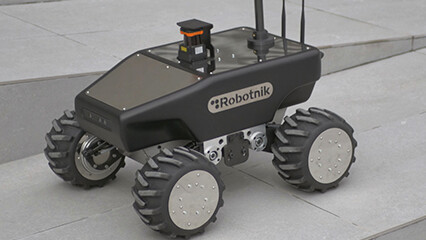
\includegraphics[width=0.6\textwidth]{imagenes/robotnik.jpg}
	\caption{Ejemplo de robot móvil autónomo - Fuente: \textit{Robotnik}}
	\label{robotnik}
\end{figure}


\section{Objetivos opcionales}

En esta sección enumeraremos y describiremos sucíntamente qué otras ideas surgieron durante el momento de \textit{brainstorming} del proyecto, y que si bien son opcionales para su desempeño, realmente aportarían algún valor al producto final.\\


\subsubsection{Movilidad autónoma}

Un factor que haría de \textbf{\textit{Lazarillo}} un producto totalmente independiente y útil sería que no necesitase de caminos guiados para desplazarse. Se valoraría la instalación en sí mismo de los mapas cerrados en que se ubicaría durante su desempeño, así como un mecanismo de \textbf{geolocalización} en el espacio. Contando con esto, el robot mantendría una comunicación persistente con el servidor informando en \textit{tiempo real} de la ubicación actual.\\






\chapter{Implementación}

En este capítulo comentaremos a fondo las decisiones tomadas que hemos comentado previamente en base a la especificación, además de describir las implementaciones propuestas con las distintas tecnologías utilizadas. Pondremos el foco no solo en el \textbf{software implícito en el robot} sino también a los componentes desarrollados externos a él, pero que también conforman la arquitectura completa de la plataforma, como lo son el \textbf{sistema operativo}, el \textbf{panel web de administración} y otras herramientas involucradas. Las ideas que por una razón u otra no hayan llegado a implementarse a tiempo, serán definidas en profundidad en apartados posteriores.\\

Para elaborar este capítulo de una forma más legible y entendible, seguiremos una estructura muy similar a la propuesta en el capítulo 3 de \textbf{Especificación de requisitos}.\\


\section{Requisitos generales}


\subsection{Licencias y compartición del software}

En cuanto a licencias y permisos del proyecto, como se anticipó se usarán diversos \textbf{repositorios} en \textit{Github}, que aparecen listados a continuación y descritos en función del contenido (que se elaborará más tarde):

\begin{itemize}
	\item \textbf{\textit{lazarillo-embedded}}: \cite{lazarillo-embedded}
	\item \textbf{\textit{lazarillo-admin-frontend}}: \cite{lazarillo-admin-frontend}
	\item \textbf{\textit{lazarillo-admin-backend}}: \cite{lazarillo-admin-backend}
	\item \textbf{\textit{meta-lazarillo}}: \cite{meta-lazarillo}
	\item \textbf{\textit{documentacion-tfm}}: \cite{documentacion-tfm}
\end{itemize}


\section{Sistema operativo}

Para dotar a la \textit{Raspberry} de un sistema operativo ligero, extensible y hecho a medida, decidimos obviar sistemas ya existentes como \textit{Raspbian} (S.O. de culto para la mayoría de usuarios de este computador) (TODO: ref a Raspbian) y confeccionar el nuestro propio a través de una herramienta libre y gratuita como es \textit{The Yocto Project} (TODO: ref a yocto).

\subsubsection{¿Por qué omitimos un sistema operativo que ya existe?}

Pues bien, la respuesta es fácil. \textit{Raspbian} es un sistema operativo de uso general que permite utilizar la \textit{Raspberry} como cualquier ordenador normal, ya sea para ofimática, desarrollo de software, consumo de recursos multimedia o incluso videojuegos. Esto provoca que el sistema operativo en cuestión venga con demasiado \textit{bloatware} (TODO: poner en el glosario) preinstalado de base; y llevaría más tiempo modificar la imagen de \textit{Raspbian} para que no contenga todo el software no deseado que confeccionar un sistema operativo a medida.\\

Además, deseamos que el robot solo muestre una aplicación embebida en pantalla en lugar de un entorno de escritorio normal, por lo que podemos prescindir de este entorno completo y configurar nuestro nuevo sistema para que solo muestre una aplicación y ahorre tiempo en el arranque.\\


\section{Arquitectura de Lazarillo}

En esta sección enumeraremos los distintos servicios y módulos específicos creados para Lazarillo y describiremos el propósito para el que han sido programados.\\

(TODO: insertar diagrama de arquitectura)

\subsection{Servicios internos}

Veamos ahora una breve explicación del propósito que satisfacen los módulos software internos del robot.

\subsubsection{lazarillo-hmi}

La tecnología usada por esta aplicación, se ha decidido que sea el framework de \textbf{\textit{Qt}}, que pese a tener modalidades de licencias de pago, permite un uso \textit{open source}. Además, se trata de una tecnología con una amplia comunidad, una documentación muy rica y un gran soporte para dispositivos embebidos. Por otro lado, dispongo de amplia experiencia con dicha herramienta, lo que agiliza enormemente el tiempo de desarrollo.

Se trata de la aplicación que muestra la interfaz táctil al usuario.

\subsubsection{messages-definition}

Este módulo no es en sí un servicio sino una \textbf{librería} donde se definen los mensajes que utilizan internamente el resto de servicios para comunicarse.

\subsubsection{service-base}

Este módulo define el esqueleto abstracto de cada uno de los servicios del robot. Heredando el comportamiento de esta librería, cada uno de los nuevos servicios se ahorran procedimientos rutinarios como instanciar la conexión con la base de datos y el bróker de mensajería.

\subsubsection{web-gateway}

Este servicio es el \textit{puerto de entrada} a Lazarillo. Realiza la comunicación mediante \textit{Websockets} con \textbf{\textit{lazarillo-admin}}, el portal web a través del cual un técnico puede administrar los distintos robots. \textit{\textbf{Web-gateway}} actúa como intérprete de los mensajes provenientes del \textit{socket} y los publica en la mensajería interna del robot (basada en \textit{Redis}) para informar al resto de servicios de cualquier acción emitida por el servidor.


\subsection{Componentes externos}

Como venimos comentando, además del software embebido en el robot, disponemos de otros módulos externos a él que completan la plataforma.

\subsubsection{lazarillo-admin}

Este es el título asignado al servicio web que tanto venimos comentando a lo largo de este documento, a través del cual podemos visualizar y gestionar los distintos robots conectados al servidor.\\

Está programado con \textit{NodeJS} (TODO: ref a node) y utiliza librerías para hacer las veces de servidor con \textit{HTTPS} (para la web) y con \textit{Websockets} (para la comunicación con el robot).\\

\chapter{Conclusiones}


% \nocite{*}
\bibliographystyle{ieeetr}
\bibliography{bibliografia/bibliografia}

%\appendix
%\input{glosario/entradas_glosario}
% \addcontentsline{toc}{chapter}{Glosario}
% \printglossary

\end{document}
